\documentclass[11pt]{article}
\usepackage{icmlko}
\begin{document}

\title{용량을 원하는 것은 비선형을 가진 도메인이다 --- 넷째 후보가 살았다}
\author{월드모델 실험실}
\date{노트 410 · 2026년 8월 1일}
\maketitle

\begin{abstract}
노트 408·409가 축 하나를 확정했다 --- \textbf{도메인마다 원하는 용량이
따로 있고}, 기계 셋(깊이 · lr · 자루 섞기)이 $|\rho| = 0.68 \sim 0.85$ 로
같은 순서를 만든다. 그런데 설명 후보 셋이 죽었다: 크기 · 원핫 아쉬움 ·
표시자 무늬 순도.

넷째를 사전 등록했다 --- \textbf{비선형 요구}. 깊이가 사는 것은
상호작용이다. 축$\to$라벨 지도가 선형에 가까운 도메인은 깊이를 줘도 쓸 데가
없고, 비선형인 도메인은 깊이를 원한다. F6\_directpool 은 F18 과
\textbf{완전히 같은 자질}의 선형 모형이므로 그 차가 비선형의 크기다.

\begin{center}
\begin{tabular}{lr}
\hline
같은 표적(용량 선호 $=$ F18@6 $-$ F18@4)에 대고, $n{=}11$ & $\rho$ \\
\hline
크기 (유보 행) & $-0.009$ \\
표시자 무늬 순도 & $+0.067$ \\
원핫 아쉬움 & $+0.373$ \\
\textbf{비선형 요구} (F18@4 $-$ F6) & $\mathbf{+0.773}$ \\
\hline
\end{tabular}
\end{center}

\textbf{사전 등록 문턱($+0.6$)을 넘었다.} 그리고 이번엔
\textbf{공유항 검사를 통과했다} --- 비선형을 F18@\textbf{6} 으로 재면
$+0.845$ 지만 그 값은 용량 선호와 F18@6 을 \emph{양쪽에 $+$ 로} 나눠 갖는다.
F18@\textbf{4} 로 재면 공유항이 한쪽은 $+$, 한쪽은 $-$ 라 상관을
\textbf{깎는} 쪽인데도 $+0.773$ 이 남는다.
\end{abstract}

\section{아이돌이 극단이다}

아이돌의 선형 편상관은 $\mathbf{-0.0295}$ 다 --- \textbf{우연보다 못하다}.
같은 자질로 F18 은 $+0.3163$ 을 낸다. \textbf{아이돌의 신호는 전부
비선형이다.} 그래서 용량 선호도 $+0.1255$ 로 압도적 1등이고, 깊이 $4{\to}6$
관문에서 혼자 $+0.1179 \cdot 12/12$ 를 냈다(노트 406).

반대편은 팝업이다 --- 선형 $+0.4985$ 인데 F18@6 이 $+0.4462$ 로
\textbf{선형보다 낮다}. 비선형 요구가 $-0.0478$ 이고 용량 선호도 유일한
음수($-0.0045$)다. 시장팝업도 같다($-0.0189$ · $+0.0027$).
\textbf{선형으로 이미 다 설명되는 도메인에 나무를 깊게 주면 손해다.}

\section{어긋나는 하나}

웹툰은 비선형 요구가 $+0.1050$ 으로 넷째인데 용량 선호는 $+0.0020$ 으로
열째다. 노트 408·409에서 두 손잡이와 섞기 모두에서 \textbf{축의 한쪽 끝에
혼자 있던} 그 도메인이다. 비선형은 있는데 깊이를 안 원한다 --- 남은 설명은
\textbf{잡음}이겠지만 안 쟀다. 판 무게 21\% 짜리라 이 하나가 전역 깊이를
계속 끌어내린다.

\section{이것이 전이를 풀어 주지는 않는다}

용량 선호는 이제 \textbf{도메인의 성질}로 설명된다. 그런데 그 성질을 재려면
\textbf{그 도메인의 라벨이 있어야 한다}(선형과 비선형을 둘 다 적합해서
빼야 한다). 안 본 도메인에는 라벨이 없다. \textbf{노트 409가 자루 무게에서
만난 벽과 같은 벽}이다 --- 도메인별로 좋은 것을 알아도, 안 본 도메인에서는
그 값을 읽을 수가 없다.

\section{남은 것}

\begin{tabular}{lp{7.2cm}}
\hline
웹툰 & 축에서 유일하게 어긋나고 판 무게 21\% 다. 잡음인지 다른 것인지 \\
축 분포에서 읽기 & 라벨 없이 비선형 요구를 짐작할 수 있나. 되면 안 본
도메인에도 맞는 깊이를 줄 수 있다 \\
선형이 나은 도메인 & 팝업·시장팝업은 F18 이 F6 보다 낮다. 지금 판은 그
둘에게 나무를 억지로 씌우고 있다 \\
\hline
\end{tabular}

\begin{figure}[h]
\centering
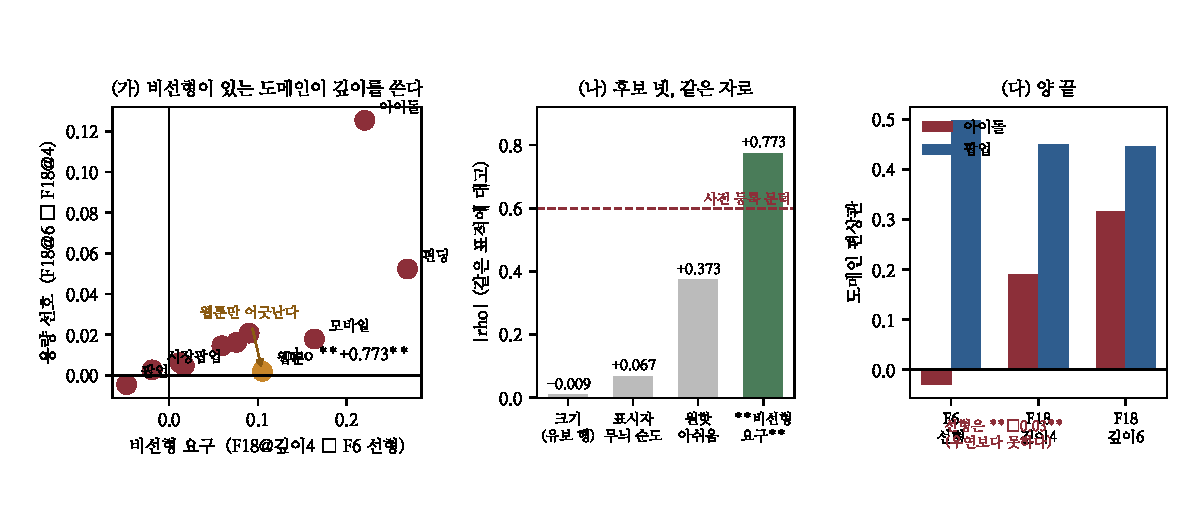
\includegraphics[width=\textwidth]{figs/fig410.pdf}
\caption{(가) 비선형 요구와 용량 선호 ($\rho = +0.773$, 공유항 검사 통과).
(나) 후보 넷을 같은 자로. (다) 양 끝 --- 아이돌은 선형이 $-0.03$ 이라
신호가 전부 비선형이고, 팝업은 깊어질수록 내린다.}
\end{figure}

\end{document}
